
\documentclass[11pt]{article}

\usepackage{common}
\usepackage{hyperref}
\title{HW2: Tagging From Scratch}
\author{Jeffrey Ling \\ jling@college.harvard.edu \and Rohil Prasad \\ prasad01@college.harvard.edu }
\begin{document}

\maketitle{}
\section{Introduction}

In this assignment, we tackle the problem of part-of-speech tagging. 

The problem can be outlined as follows. Given a set of tokenized text with each token given a tag corresponding to the part of speech that it functions as, can we train a model that can read in other sets of tokenized text and accurately determine the part of speech for every word? 

We will train our models on a tagged excerpt from the Wall Street Journal and test them on another, i.e. the Penn Treebank dataset. We examine three different models for this purpose. These three models are multinomial naive Bayes, logistic regression, and the neural network from Collobert et al (2011).

In Section $2$, we introduce our notation and give a description of our problem in formal language. In Section $3$, we describe our three models. In Section $4$, we present our experimental results for model performance and hyperparamater tuning. In Section $5$, we conclude with a discussion of our results. 

\section{Problem Description}

Our raw data consists of pairs $(w_i, t_i) \in \mcV \times \mcT$ for $i = 1, \ldots, N$ where $N$ is our data size, where $w_i \in \mcV$ is a word in our corpus and $t_i$ is its corresponding part of speech (POS) tag. The $t_i$ are elements of a finite set of classes $\mcT$, which we take as the list of POS tags provided in the homework. Example POS tags are NNP, VBD, VBZ, etc. and in this problem we have a total of $|\mcT| = 45$ tags.

We construct a feature representation of each word $w$ as follows. 

First, construct the vocabulary $\mcV$ of the training and testing sets. To keep this from growing too large, we only use lower-case words. Furthermore, we map any uncommon words to a special ``RARE'' word, where we use the words in the publicly available data from the Glove word embeddings as our ``common words'' dictionary. A word $w$ then can be associated with a sparse one-hot feature vector $\boldj \in \{0,1\}^{|\mcV|}$, with 1 at the index $j$ that $w$ maps to in $\mcV$ (where $j = 1, \ldots, |\mcV|$). 

Second, we can also construct a feature $c \in \mcC$ that keeps track of the capitalization information in $w$ that we lost above when we made it lowercase. This feature is dependent on if $w$ is all lowercase, all uppercase, starts with an uppercase letter, or contains an uppercase letter, in that order of priority, thus giving $|\mcC| = 4$. We represent this feature for $w$ with a sparse one-hot feature vector $\boldc \in \{0,1\}^\mcC$.

Finally, we add context by not only adding in the features of $w_i$, but also adding in the features of the words in a \emph{window} around $w_i$. In our case, we use a fixed window of size $5$, so our data sample becomes $\boldx_{i, word} = \{\boldj_{i-2}, \boldj_{i-1}, \boldj_i, \boldj_{i+1}, \boldj_{i+2}\} \in \{0,1 \}^{5|\mcV|}$ and $\boldx_{i, cap} = \{\boldc_{i-2}, \boldc_{i-1}, \boldc_i, \boldc_{i+1}, \boldc_{i+2}\} \in \{0,1\}^{5|\mcC|}$ of vocabulary and capitalization features corresponding to the surrounding word window, and we will denote these features $(\boldx_{i, word}, \boldx_{i, cap})$ by $\boldw_i$.

If the window overlaps the start or end of the sentence, we represent the words as a vector of all zeroes.

Our goal is thus to learn a function $f: \{0,1\}^{5|\mcV|} \times \{0,1\}^{5|\mcC|} \to \mathbb{R}^|\mcT|$ that takes in a window of words $\boldw$ and outputs a prediction vector $\hat{\boldy}$ where $\hat{y}_k$ is the log probability $\log p(t|w_i)$ of the middle word $w_i$ of $\boldw_i$ having tag $i$.

\subsection{Practice}

In practice, we simply represent a word $w \in \mcV$ with its index $j$ where $j = 1, \ldots |\mcV|$, and similarly represent its feature $c \in \mcC$ with the index $j_c = 1, \ldots, |\mcC|$. The \texttt{nn.LookupTable} function in Torch allows us to perform the matrix operation $\boldj W$ by simply sparsely indexing into the $j$th row of $W$, and we do the same for the capitalization features.

\subsection{Extension: Suffix Features}

As an extension to the baseline model described in Collobert et al, we add in suffix features as well. We merely take for a word $w$ its last two letters $s \in \mcS$ where $\mcS$ is the set of word suffixes. We can then derive features $\bolds \in \{0, 1\}^\mcS$ for word $w$ and $\boldx_{i, suffix} \in \{0, 1\}^{5|\mcS|}$ for a window of words centered at $i$ just as described before, and concatenate them to the feature representation.

Again, in practice we store the index $j_s = 1, \ldots, |\mcS|$ for word $w$, and use \texttt{nn.LookupTable}.

\section{Model and Algorithms}

We use three models:
\begin{itemize}
  \item multinomial naive Bayes (MNB)
  \item logistic regression
  \item neural network from Collobert et al (2011)
\end{itemize}

Below we describe the setup of each.

\subsection{Multinomial Naive Bayes}

In MNB, we assume that the features of a word window $\boldw$ are independent of each other. 

We can apply Bayes' law to calculate the probability $p(t| \boldw)$ of class $t$ given $\boldw$. 
$$p(t| \boldw) = \frac{p(t)p(\boldw |t)}{p(\boldw)}$$

Our prediction $\hat{y}$ for $\boldw$ is given by the maximum-probability tag
$$\hat{y} = \argmax_{t} p(t | x)$$

Note that $\boldw$ is a window of words. Assuming that the middle word is equal to $w_i$, we can apply our independence assumption to get 

$$p(t | \boldw) = \frac{p(t)\prod_{d=-2}^{d=2} p(w_{i+d} | t)}{\prod_{d=-2}^{d=2} p(w_{i+d})}$$

The $p(w_{i+d})$ are constant functions of the output $t$, so we can focus on calculating the terms in the numerator. 

Recall that every word $w$ can be represented as a two sets of binary values $e_1, \dots, e_{|\mcV|}$ and $e^{cap}_1, \dots, e^{cap}_{|c|}$. By our independence assumption, we have 
$$p(w | t) = p(e_1, \dots, e_{|\mcV|}, e^{cap}_1, \dots, e^{cap}_{|\mcC|} | t) = \prod_{m=1}^{|\mcV|} p(e_m | t) \prod_{n=1}^{|\mcC|} p(e^{cap}_n | t)$$

Therefore, it suffices to maximize the $p(e_m | t)$ and $p(e^{cap}_n | t)$. Under negative log-likelihood loss, these are maximized over the entire training set by counting the number of samples with tag $t$ that have word feature $e_m$ and capitalization feature $e^{cap}_n$ respectively and then dividing by the total number of samples with tag $t$. 

The maximum likelihood estimate for $p(t)$ is the proportion of samples with tag $t$. 

Overall, our prediction becomes
$$\hat{y} = \argmax_t \sum_d (\sum_m \log p(e_m | t) + \sum_n \log p(e^{cap}_n | t)) + \log p(t)$$
where the sum is taken over all words in the window $\boldw$. 

\subsection{Logistic Regression}

We assume a linear model $z = \boldx_{word} \boldW + \boldx_{cap} \boldW_{cap} + \boldb$, where $\boldx_{word}$ and $\boldx_{cap}$ are the word and capitalization features of an input word window $\boldw$. 

We then apply the softmax function to get an output $\hat{\boldy}$, where $\hat{y}_t$ is the predicted probability for a tag $t$ given the window $\boldw$. 
%
%This is implemented using the following neural network architecture:
%(Picture)

The parameters are optimized via stochastic gradient descent and a negative log-likelihood criterion like in our last assignment. 

\subsection{Neural Network}

The neural network model of Collobert et al (2011) simply stacks more functions before the softmax in logistic regression. A diagram:


\begin{figure}
\centering
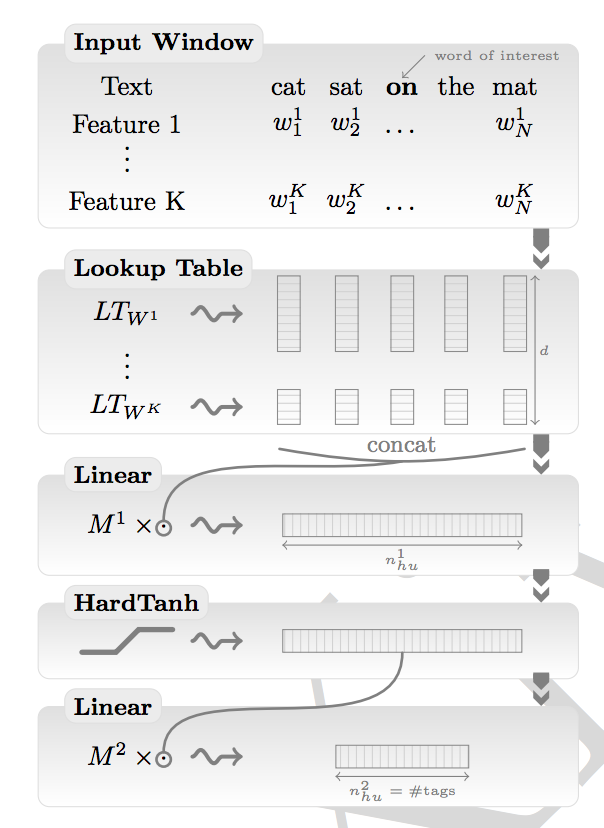
\includegraphics[scale=0.5]{collobert_network}
\caption{Neural network architecture of Collobert et al.}
\end{figure}

The first layer of the model performs a matrix multiplication for each one-hot $\boldj_i$ as $\boldj_iW_{0, word}$, where $W_{0, word}$ is a $|\mcV|$ by $d_{word}$ to get a word embedding $\bolde_i \in \mathbb{R}^{d_{word}}$. Here, $d_{word}$ is a hyperparameter that can be chosen.

We do the same with a weight matrix $W_{0, cap}$ of size $|\mcC|$ by $d_{cap}$ on $\boldc_i$ to get a capitalization vector $\bolde_{i, cap} \in \mathbb{R}^{d_{cap}}$.

Thus the input $(\boldx_{word}, \boldx_{cap})$ is transformed into a pair
$$[\bolde_{i-2}, \bolde_{i-1}, \bolde_{i}, \bolde_{i+1}, \bolde_{i+2}] \in \mathbb{R}^{5d_{word}}$$
$$[\bolde_{i-2, cap}, \bolde_{i-1, cap}, \bolde_{i, cap}, \bolde_{i+1, cap}, \bolde_{i+2, cap}] \in \mathbb{R}^{5d_{cap}}$$

Let us represent the concatenation as $\boldz_{0, i} \in \mathbb{R}^{5d_{word} + 5d_{cap}}$. We then perform a linear transformation with matrix $W_1$ of size $5d_{word} + 5d_{cap}$ by $h$, where $h$ is a hyperparameter that's the number of hidden layers, and also use a bias term $b_1 \in \mathbb{R}^h$ to get a result $\boldz_{1,i} \in \mathbb{R}^h$.
$$\boldz_{1,i} = \boldz_{0,i}W_1 + b_1$$

We then perform the hard tanh activation function termwise, which is defined as
$$HardTanh(x) = \begin{cases} -1 & x < -1 \\ x & -1 \leq x \leq 1 \\ 1 & x > 1 \end{cases}$$

Finally, we perform a linear transformation with matrix $W_2$ of size $h$ by $|\mcT|$ to get the desired output $\boldz_{2,i} \in \mathbb{R}^{|\mcT|}$. The last step is a log softmax.
$$\boldz_{2,i} = HardTanh(\boldz_{1,i})W_2 + b_2$$
$$\widehat{\boldy_i} = LogSoftMax(\boldz_{2,i})$$

We also optimize the parameters with SGD and backpropagation.

\subsubsection{Glove Embeddings}

Glove word embeddings are pretrained word vectors from Pennington et al (2014). We can initialize our word embedding parameters in the neural network architecture with these word embeddings to obtain better results, since we hope that SGD will reach a better local optimum in the parameter space with previous substructure.

%\begin{itemize}
%\item diagrams of your model,
%
%  \begin{center}
%    \includegraphics[width=0.4\textwidth]{network}
%  \end{center}
%\item feature tables,
%
%  \begin{center}
%    \begin{tabular}{@{}lll@{}}
%      \toprule
%      &\multicolumn{2}{c}{Mention Features  } \\
%      & Feature & Value Set\\
%      \midrule
%      & Mention Head & $\mcV$ \\
%      & Mention First Word & $\mcV$ \\
%      & Mention Last Word & $\mcV$ \\
%      & Word Preceding Mention & $\mcV$ \\
%      & Word Following Mention & $\mcV$\\
%      & \# Words in Mention & $\{1, 2, \ldots \}$ \\
%      & Mention Type & $\mathcal{T}$ \\
%      \bottomrule
%    \end{tabular}
%  \end{center}
%
%\item pseudo-code,
%
%  \begin{algorithmic}[1]
%    \Procedure{Linearize}{$x_1\ldots x_N$, $K$, $g$}
%    \State{$B_0 \gets \langle (\langle \rangle, \{1, \ldots, N\}, 0, \boldh_0, \mathbf{0})  \rangle$}
%    \For{$m = 0, \ldots, M-1$ }
%    \For{$k = 1, \ldots, |B_m|$}
%    \For{$i \in \mcR$}
%    \State{$(y, \mcR, s, \boldh) \gets \mathrm{copy}(B_m^{(k)})$}
%    \For{word $w$ in phrase $x_i$}
%    \State{$y \gets y $ append $w$ }
%    \State{$s \gets s + \log q(w, \boldh) $ }
%    \State{$\boldh \gets \delta(w, \boldh)$}
%    \EndFor{}
%    \State{$B_{m+|w_i|} \gets B_{m+|w_i|} + (y, \mcR - i, s,   \boldh)$}
%    \State{keep top-$K$ of $B_{m+|w_i|}$ by $f(x, y) + g(\mcR)$}
%    \EndFor{}
%    \EndFor{}
%    \EndFor{}
%    \State{\Return{$B_{M}^{(k)}$}}
%    \EndProcedure{}
%  \end{algorithmic}
%
%\end{itemize}

\subsection{Training Methods}

We ran vanilla batch stochastic gradient descent on training and validation sets. For batches, we shuffled the training set once and iterated over it for each epoch. For preliminary results we ran SGD for at least 5 epochs, and then stopped when relative validation loss (defined as the fractional change in validation loss) dropped below $0.1\%$.

We continued training on the neural model (with Glove word embeddings) when it was clear that the model had not completed training with this criterion. The use of validation error rather than training error prevents overfitting.

\section{Experiments}

We ran batch SGD for maximum 20 epochs with batch size 32 and learning rate 0.01. For naive Bayes we used $\alpha = 1$. For neural models, we used word embedding dimension 50, capitalization feature embedding dimension 5, and hidden layer size 300 (as in Collobert et al). We ran most experiments on Odyssey with 16GB memory.

We didn't extensively tune hyperparameters in this experiment, but rather tried different model setups.

Training time tended to vary for each model depending on the Odyssey server it ran on and time of day. Table~\ref{tab:timings} gives some ballpark timing results for each model.

\begin{table}[h]
\centering
\begin{tabular}{llr}
 \toprule
 Model &  & Timing \\
 \midrule
 \textsc{Naive Bayes} & & 16 s\\
 \textsc{Logistic Regression (per epoch)} & & 10 min \\
 \textsc{Neural (per epoch)} & &12 min \\
 \bottomrule
\end{tabular}
\caption{\label{tab:timings} Timing results on PTB training.}
\end{table}

For reference, the PTB dataset has 950885 training points, so a batch size of 32 gives a training time of 24.2 ms per batch. 

Figure ~\ref{fig:loss} shows the training and validation loss over epochs for the neural model with Glove word embeddings. Note that loss consistently decreases, and we stopped training when validation loss stopped decreasing. The bump in the validation accuracy is from when we restart training from a saved model, and is possibly due to a new batch shuffle for training.

\begin{figure}
	\centering
	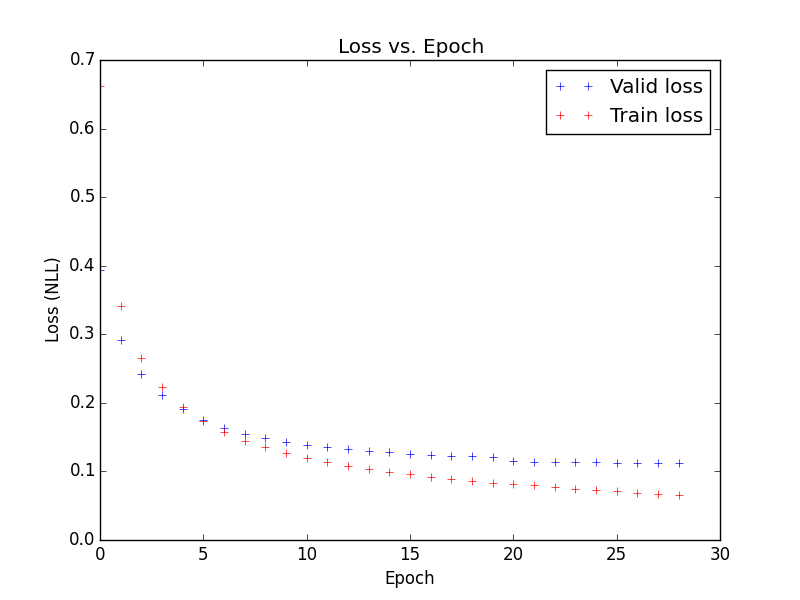
\includegraphics[scale=0.4]{loss_plots}
	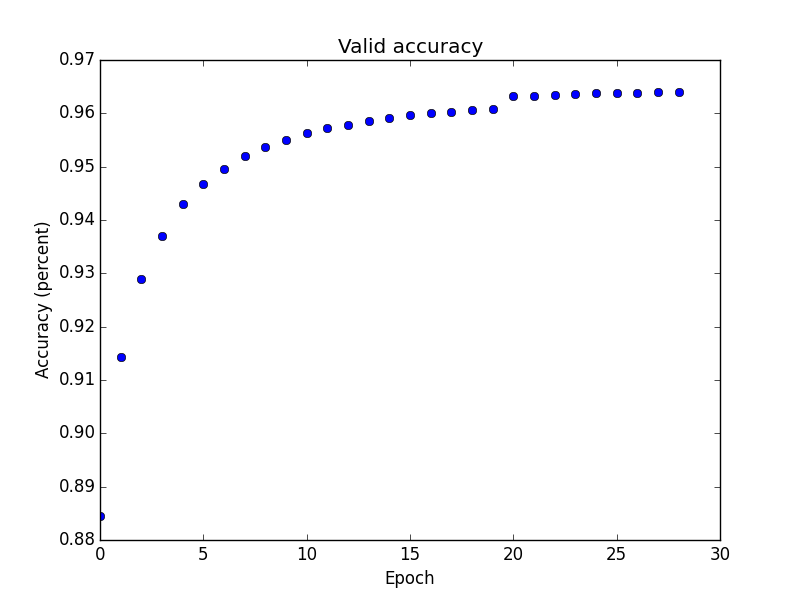
\includegraphics[scale=0.4]{acc_plot}
	\caption{\label{fig:loss} Training curves.}
\end{figure}

We found that after 20 epochs, the neural model with pretrained word embeddings had the best validation rate, but training had not yet converged. Thus, we ran it for about 10 more epochs until the validation error stopped decreasing.

Table~\ref{tab:results} gives the classification accuracy of each model on the validation set. The results shown are after training 20 epochs, except for models with Glove embeddings (which we trained for longer). For neural models, GLOVE means we used pretrained Glove word embeddings and SUFF means we included suffix features.

\begin{table}[h]
\centering
\begin{tabular}{llr}
 \toprule
 Model &  & Acc. \\
 \midrule
 \textsc{Naive Bayes} & & 91.27\\
 \textsc{Naive Bayes (no cap features)} & & 89.98 \\
 \textsc{Logistic Regression} & & 76.50 \\
 \textsc{Neural} & & 92.11  \\
 \textsc{Neural+GLOVE} & &96.41 \\
 \textsc{Neural+GLOVE+SUFF} & & 96.60 \\
 \bottomrule
\end{tabular}
\caption{\label{tab:results} Results on PTB POS tagging.}
\end{table}

For naive Bayes, we tried including and excluding the capitalization features, and it turns out that capitalization gives better accuracy as expected. The model with suffixes included does the best, suggesting that more features should be experimented with to retrieve more signal.


As an extension, we also tried to run Adadelta instead of SGD. However, because it saves $O(P)$ values for each iteration, where $P$ is the number of parameters in the model, it turns out to be prohibitively expensive for memory, and training did not finish in time.

\section{Conclusion}

In this homework, we built a POS tagger by preprocessing the PTB text corpus into window-sized data points. Then we ran baseline models of naive Bayes and logistic regression, and finally applied the neural network model of Collobert et al (2011).

We found that training these neural models takes a significant amount of time, and thus careful logging and saving models after each epoch was important, allowing us to restart training at any checkpoint. Running on Odyssey also helped by offloading computation to a cloud server. We expect that with GPUs, training these models will be much quicker and easier.

Also since restarting training with a new batch shuffle seems to change validation accuracy fairly significantly, we should probably shuffle the batches each time.

The code for this homework can be found here: \url{https://github.com/r0hilp/cs287-hw2}

\bibliographystyle{apalike}
\bibliography{writeup}

\end{document}
